% !TeX root = Tesis.tex
% !TeX encoding = UTF-8
% !TeX spellcheck = es_CU-SpanishCuba
\chapter{Resultados}
\label{cap3}
\onehalfspacing

\section{Principales resultados}

Sobre la base de nuestros diagramas, podemos formular las siguientes observaciones o afirmaciones, que son los principales resultados del trabajo.

\begin{enumerate}
	\item  \textbf{Existe una dirección en el espacio de expresión genética, que a grandes rasgos se puede identificar con el eje PC1, asociada al envejecimiento y a un aumento del riesgo de padecer GB y la EA.}
\end{enumerate}

De hecho, el desplazamiento en esta dirección implica escalar parcialmente las barreras de bajo \textit{fitness} que separa N de los estados GB y EA, y por lo tanto aumentar el riesgo tanto para GB como para la EA.

Vale la pena observar los principales genes involucrados en este proceso. Para ello, observamos el vector unitario a lo largo del eje PC1. Los genes se clasifican según su contribución al vector unitario.% \alert{El procedimiento es similar al algoritmo de Page Rank \cite{Duhan_2009}. Lo usamos en nuestro trabajo anterior \cite{Gonzalez_2023}.}

En la Tabla \ref{tab:apx3} de los apéndices se encuentra una lista con los 100 primeros genes del \textit{ranking}. En la Fig. \ref{fig:figpc1} se representan los valores de los 30 primeros genes en el vector PC1 ordenados por su valor absoluto. Las amplitudes positivas definen genes cuya expresión aumenta con el desplazamiento a lo largo de la dirección positiva de PC1, mientras que las amplitudes negativas se refieren a genes silenciados. Estos genes deberían desempeñar simultáneamente un papel crucial en el envejecimiento, el GB y la EA.

\begin{figure}[!htb]
	\centering
	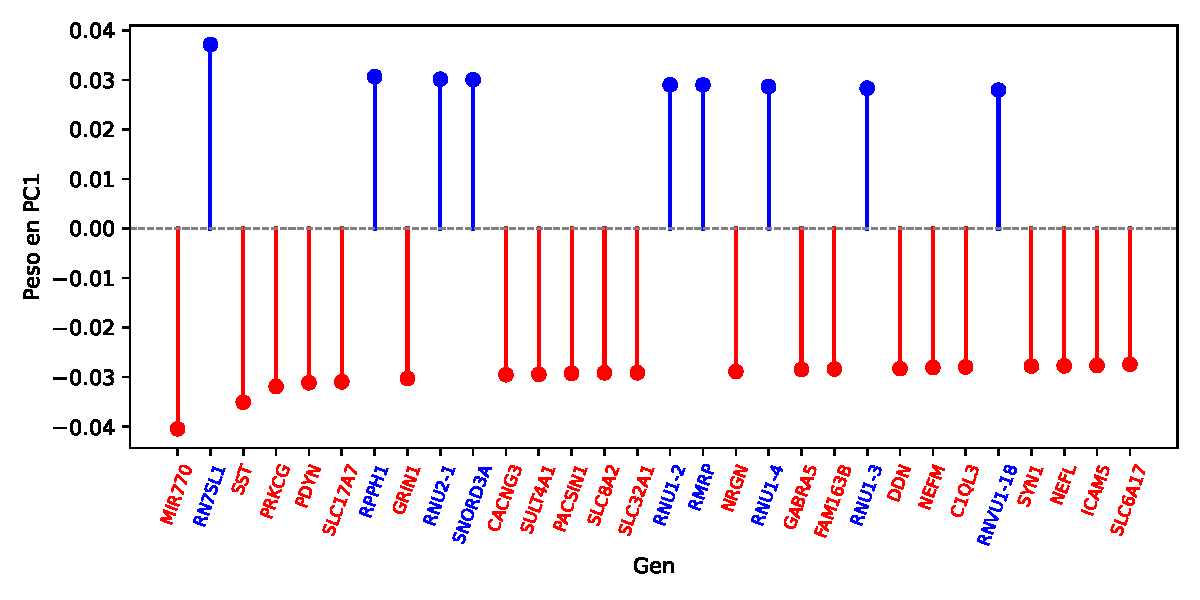
\includegraphics[width=\linewidth]{figures/PC1}
	\caption{Genes con mayor peso a lo largo del vector PC1.}
	\label{fig:figpc1}
\end{figure}

Por supuesto, debido al valor puramente cualitativo de nuestro análisis, los genes, y especialmente el \textit{ranking}, deben considerarse con cautela. Sin embargo, cabe destacar que 20 de los genes silenciados están relacionados con los procesos principales de transmisión a través de sinapsis químicas. En la Tabla \ref{tab:apx4} del Apéndice \ref{apx:apx3} se enumeran los procesos principales del \textit{Reactome} (\href{https://reactome.org/}{https://reactome.org/}) asociadas a estos genes \cite{Gillespie_2021}. Este conjunto incluye 56 genes anotados.

La disminución de la función sináptica es una característica conocida del cerebro envejecido, según la revisión \cite{Ham_2020}. La segunda característica principal, según esta referencia, es un aumento de la función inmunitaria, que no es particularmente evidente en nuestro conjunto de genes. En cambio, observamos genes relacionados con la neurotoxicidad de las toxinas de clostridium \cite{Biazzo_2022}, con la disminución de la actividad mitocondrial \cite{Sun_2016}, micro ARN compartidos entre la EA y el GB \cite{Thomas_2020}, etc.

\begin{enumerate}
	\item[2.] \textbf{Hay una dirección en el espacio de expresión genética, que puede identificarse aproximadamente con el eje PC2, que muestra que la EA y GB son alternativas excluyentes.}
\end{enumerate}

De hecho, la EA y el GB aparecen en semiplanos opuestos. La evidencia clínica \cite{ou2012does, Driver_2012, Roe_2010, Musicco_2013} y los estudios de biología molecular \cite{Liu_2013, Lanni_2020} respaldan esta disyunción. En consecuencia, el eje PC2 involucra genes con desregulación inversa en la EA y el GB.

En la Tabla \ref{tab:apx5} de los apéndices, se listan los 100 genes principales definidos por el vector unitario a lo largo del eje PC2. En la Fig. \ref{fig:figpc2} se representa gráficamente la contribución a dicho vector de los 30 primeros genes ordenados por su valor absoluto. Los pesos positivos corresponden a genes cuya expresión aumenta en la transición de N a la EA. Por otro lado, las amplitudes negativas corresponden a genes cuya expresión aumenta en la transición de N a GB.

\begin{figure}[!htb]
	\centering
	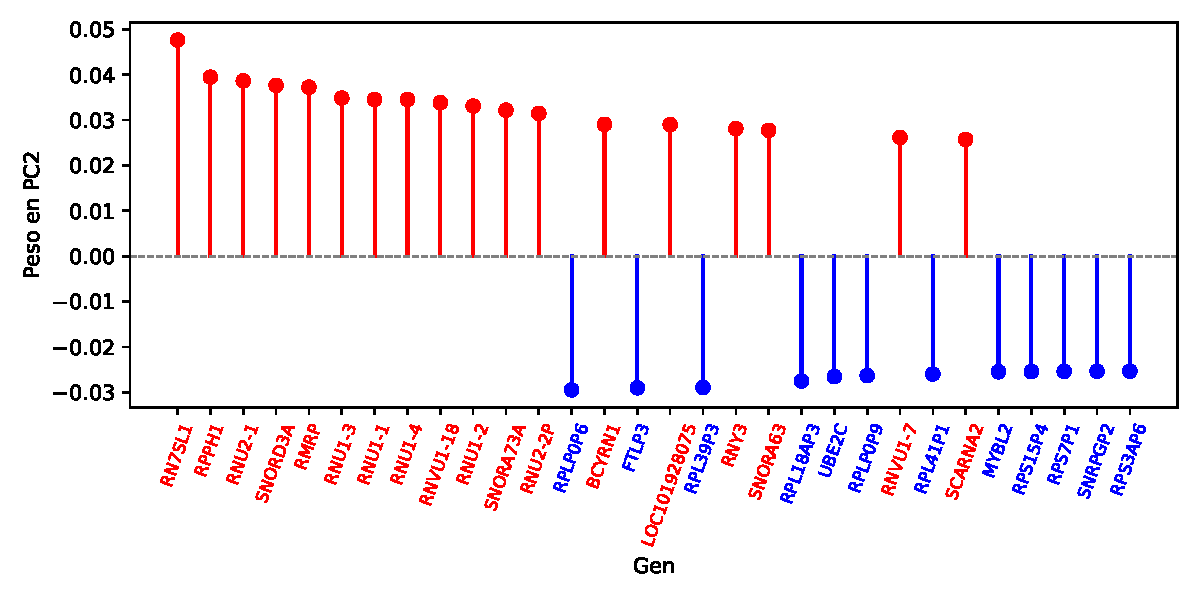
\includegraphics[width=\linewidth]{figures/PC2}
	\caption{Genes con mayor peso a lo largo del vector PC2.}
	\label{fig:figpc2}
\end{figure}

Los procesos de \textit{Reactome} relacionadas con estos genes se muestran en la Tabla \ref{tab:apx6} del Apéndice \ref{apx:apx5}. Se relacionan principalmente con el control del ciclo celular, la replicación del ADN, la apoptosis, la modificación de la matriz extracelular, etc., es decir, con las características distintivas del cáncer \cite{Hanahan_2000, Hanahan_2011, Hanahan_2022}.

Anteriormente, mencionamos MMP9 como un ejemplo de genes que desempeñan funciones opuestas en el GB y la EA. El gen codificador de la proteína UBE2C es otro gen conocido con esta característica \cite{MA_2016, Jaladanki_2021}. Por otro lado, el gen BCYRN1, también entre los primeros 100 genes del \textit{ranking}, parece estar subexpresado en GB \cite{Mu2021} y sobreexpresado en la EA \cite{Zhang_2021}. La Fig. \ref{fig:fig1d} muestra gráficos de violín para la expresión diferencial de los genes MMP9 y BCYRN1 en muestras de N, GB y la EA.

\begin{figure}[!htb]
	\centering
	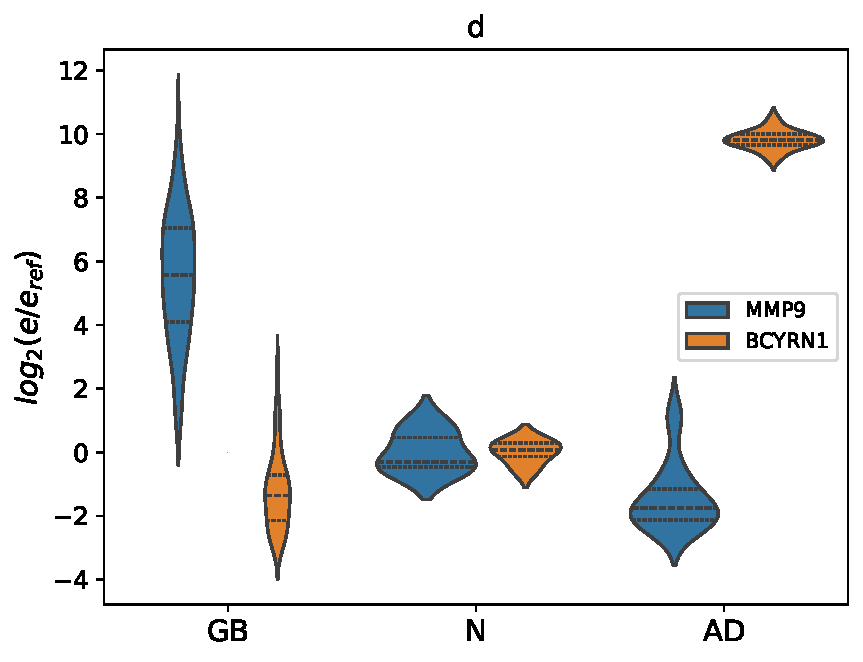
\includegraphics[width=0.75\linewidth]{figures/Fig_1d.pdf}
	\caption{Gráficos de violín para la expresión diferencial logarítmica de los genes MMP9 y BCYRN1 en los estados N, GB y EA.}
	\label{fig:fig1d}
\end{figure}

Noté también que en la Tabla \ref{tab:apx5} hay numerosos genes codificadores de proteínas ribosomales, de núcleo pequeño, de microARN y de otros tipos, regulados inversamente en ambos procesos. Solo 18 de este conjunto de genes están anotados en los procesos \textit{Reactome}. Este es un problema habitual en el análisis de procesos, donde las funciones biológicas de muchos genes no están anotadas.

\begin{enumerate}
	\item[3.] \textbf{Existe un corredor de envejecimiento, es decir un camino preferencial para el envejecimiento en el espacio de expresión genética.}
\end{enumerate}

En nuestros datos, existen muestras en la región N y muestras correspondientes a cerebros de edad normal, ubicadas en una región definida cerca del atractor de la EA. En otras palabras, el proceso de envejecimiento parece definir una trayectoria o corredor de decrecimiento continuo del \textit{fitness}, del cual los datos O muestran el último segmento. Sin embargo, faltan muestras en la región intermedia.

En lugar de incluir muestras adicionales en nuestra figura, lo cual introduciría efectos de lote adicionales, utilizamos resultados recientes en un modelo de ratón \cite{hahn2023atlas} que muestran indudablemente un corredor continuo para el envejecimiento. Presentamos en la Fig. \ref{fig:suppl1} del Apéndice \ref{apx:apx1} una representación gráfica de sus datos para el cuerpo calloso, una región rica en materia blanca. En el panel izquierdo, se grafican las dos primeras componentes principales para los centros de los subgrupos de muestras. Se consideran edades de ratón entre 3 y 28 meses; este último equivale aproximadamente a 80 años en una escala humana. Un corredor para el envejecimiento es evidente. El panel derecho, por otro lado, muestra distancias reales incluyendo todos los componentes. Por lo tanto, las proyecciones en el plano (PC1, PC2) son una representación fiel de la distribución real de puntos.

En nuestro esquema (Fig. \ref{fig:fig1b}), se delinea un corredor de envejecimiento. La Fig. \ref{fig:fig1c} sugiere que este corredor es una dirección con una mínima disminución del \textit{fitness}.

Una dirección o corredor preferencial para el envejecimiento es consistente con la hipótesis del envejecimiento programado \cite{Magalh_es_2012, Gems_2022}, es decir, la idea de que el envejecimiento está programado en nuestros genes.

\begin{enumerate}
	\item[4.] \textbf{El corredor de envejecimiento predeterminado podría estar relacionado con la presión de evitar el fuerte atractor GB.}
\end{enumerate}

Una pregunta muy interesante se refiere a la selección de la dirección preferida para el envejecimiento. Nuestro esquema simplificado (Fig. \ref{fig:fig1c}) ofrece una respuesta inesperada: en la materia blanca, esta dirección podría estar relacionada con la presión para evitar el atractor GB más fuerte.

De hecho, para cada pequeña porción de tejido, se puede modelar el envejecimiento como una especie de movimiento aleatorio que comienza en la región N. Obsérvese que en la referencia \cite{Herrero_2022} se utilizó un modelo de saltos aleatorios en el espacio de expresión genética para describir la evolución somática de diferentes tejidos hacia el cáncer. Primero, asumimos que la dirección de los saltos es aleatoria en el plano que se muestra en la Fig. \ref{fig:fig1c}.

Solo existen cuatro posibilidades para el destino de las trayectorias aleatorias en el plano que comienzan en la región N. Primero, la trayectoria permanece en la región N. Segundo, llega a una región de \textit{fitness} muy baja y las células mueren. Este es el destino de muchas células en el cerebro envejecido. Tercero, es capturada por el atractor GB. Y, finalmente, la cuarta posibilidad es la captura por el atractor de la EA.

Debido al elevado valor de \textit{fitness} del atractor GB, debería existir una probabilidad relativamente alta de que las trayectorias sean capturadas por el GB, lo que conduce a la iniciación de un tumor. Esto implica un enorme aumento del \textit{fitness}, la propagación del tumor en el cerebro y una esperanza de vida para el individuo de tan solo unos dos años tras la iniciación \cite{Poon_2020}. Esto podría afectar a los individuos en edad reproductiva. Por lo tanto, evitar el atractor GB podría ser objeto de la presión selectiva.

Como comprobación indirecta, podemos comparar las incidencias de GB y la EA. Estas deberían ser proporcionales a las tasas de captura de trayectorias aleatorias por los atractores de GB y EA. Como se mencionó, en un modelo donde la dirección de los saltos es aleatoria, la incidencia de GB debería ser mucho mayor que la de la EA. Sin embargo, la incidencia global del glioblastoma es inferior a 10 por 100 000 personas \cite{Ohgaki2005}, en contraste con el 5 \% de la EA en personas de 65 a 74 años y el 13 \% en personas de 75 a 84 años \cite{alz2023}. La incidencia observada sugiere que se evita el movimiento hacia el centro de GB.

\begin{enumerate}
	\item[5.] \textbf{La aparición tardía de la EA podría ser el resultado de la captura por parte del atractor de la EA de microestados cerebrales envejecidos.}
\end{enumerate}

La imagen es, por lo tanto, la siguiente. El proceso de envejecimiento se relaciona inicialmente con un desplazamiento a lo largo del corredor de envejecimiento, con la correspondiente disminución del \textit{fitness}. En los últimos pasos, los estados O son capturados por el atractor débil de la EA.

Como se mencionó anteriormente, la afirmación sobre el corredor de envejecimiento está respaldada por el experimento en un modelo de ratón, mientras que la captura por parte del centro de la EA está sugerida por los cálculos de la referencia \cite{Gonzalez_2021}, particularmente por los resultados que se muestran en la Fig. \ref{fig:otoad}, que es un reconstrucción de la Fig. 4 de esa referencia.

En la Tabla \ref{tab:apx7} se muestran los 10 genes principales en la transición de O a la EA. Se trata de genes incluidos en la Tabla \ref{tab:apx3}, pero que varían en dirección opuesta, es decir, en la dirección negativa del eje PC1. Este hecho se representa en el diagrama esquemático de la Fig. \ref{fig:fig1b}.


\section{Perspectiva cuantitativa}

Debido al carácter cualitativo de nuestro estudio, el análisis de genes y procesos relevantes no se aborda adecuadamente en este trabajo. Sin embargo, analicemos cualitativamente siete marcadores conocidos para la EA y el GB según nuestro esquema. Los gráficos de violín para estos genes se muestran en Fig. \ref{fig:violin}. La figura muestra que los genes MAPT (proteína tau \cite{Strang_2019}) y APP (beta amiloide \cite{TCW_2016}) están subexpresados tanto en el GB como en la EA y, por lo tanto, según nuestro esquema, son genes tipo PC1, principalmente relacionados con el envejecimiento. En cierto modo, esto concuerda con los hallazgos del estudio del Instituto Allen sobre los patrones de proteína tau y placas amiloides en el cerebro envejecido. Por supuesto, ciertas mutaciones de estos genes podrían conducir a un envejecimiento cerebral acelerado y a la aparición temprana de la EA. El gen APOE \cite{Raulin_2022}, por el contrario, está desregulado inversamente en el GB y la EA. Es un gen del tipo PC2.

\begin{figure}[!htb]
	\centering
	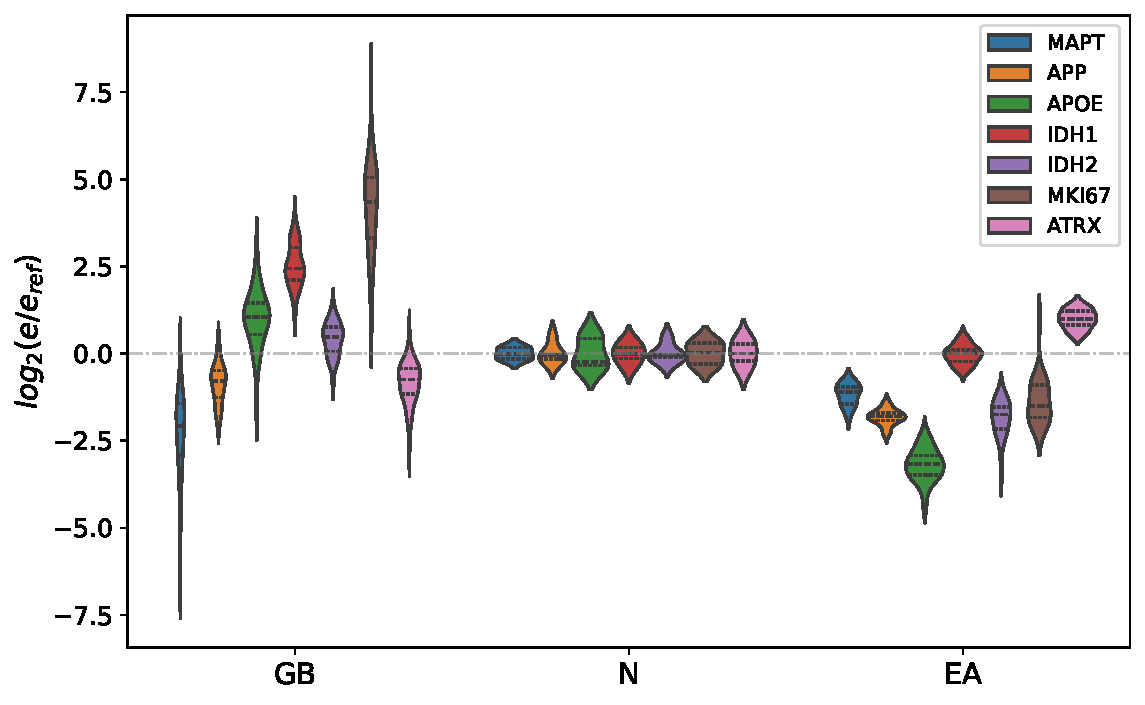
\includegraphics[width=\linewidth]{figures/suppl2}
	\caption{Gráficos de violín para marcadores conocidos en la EA y el GB.}
	\label{fig:violin}
\end{figure}

Por otro lado, el marcador IDH1 \cite{Cohen_2013} está sobreexpresado en la GB, pero es irrelevante en la EA. Los tres marcadores de GB, IDH2 \cite{Cohen_2013}, MKI67 \cite{Chen_2015} y ATRX \cite{Haase_2018}, son genes similares a PC2. Se han estudiado principalmente en relación con la GB, pero el hecho de que sean genes PC2 indica que podrían desempeñar un papel importante también en la EA.

Consideremos, como último ejemplo, la reciente demostración de la relevancia de TREM2 en la EA \cite{van_Lengerich_2023}. Se ha demostrado que la activación de TREM2 en la EA mejora el metabolismo microglial. Según nuestro análisis, TREM2 es un gen PC2, subexpresado en la EA y sobreexpresado en el GB. Por lo tanto, esperamos que la inhibición de TREM2 en células de glioblastoma pueda tener un efecto importante en el GB. Este hecho, según nuestro sencillo esquema, se encuentra actualmente en estudio \cite{Sun_2023}.

